\documentclass[11pt,a4paper]{article}

% --- PAQUETES PRINCIPALES ---
\usepackage[utf8]{inputenc}
\usepackage[T1]{fontenc}
\usepackage[spanish,es-tabla]{babel}
\usepackage{mathptmx}
\usepackage{courier}
\usepackage{float}
\usepackage[margin=2.5cm]{geometry}
\usepackage{graphicx}
\usepackage{booktabs}
\usepackage{array}
\usepackage{amsmath}
\usepackage{tabularx}
\usepackage{xcolor}
\usepackage{hyperref}
\usepackage{xurl}
\usepackage{enumitem}
\usepackage{tcolorbox}
\usepackage{listings}
\usepackage{placeins}
\usepackage{caption}
\usepackage{subcaption}
\usepackage{tikz}
\usetikzlibrary{babel,arrows.meta,positioning,fit,backgrounds,calc}
\usepackage{pgfplots}
\pgfplotsset{compat=1.16}

\definecolor{primarycolor}{gray}{0}
\definecolor{mongocolor}{gray}{0}
\definecolor{cassandracolor}{gray}{0}
\definecolor{neocolor}{gray}{0}
\definecolor{airflowcolor}{gray}{0}
\definecolor{neutralcolor}{gray}{0.35}

\captionsetup{font=small,labelfont=bf}
\setlist{itemsep=2pt,topsep=4pt}
\renewcommand{\arraystretch}{1.15}

\newcommand{\code}[1]{\detokenize{#1}}

\lstdefinestyle{celda}{
    basicstyle=\ttfamily\footnotesize,
    frame=single,
    breaklines=true,
    postbreak=\mbox{$\hookrightarrow$\space},
    breakatwhitespace=false,
    showstringspaces=false,
    columns=fullflexible,
    keepspaces=true,
    aboveskip=6pt,
    belowskip=6pt,
    xleftmargin=6pt,
    xrightmargin=6pt
}
\lstset{style=celda}
\hypersetup{hidelinks}
\urlstyle{same}
\DeclareUrlCommand\path{\urlstyle{same}}

% Estilos comunes de los diagramas
\tikzset{
    box/.style={draw=#1, fill=#1!10, rounded corners=3pt, align=center,
                font=\small, inner sep=5pt, minimum height=0.9cm, thick},
    box/.default=primarycolor,
    flow/.style={-{Stealth[length=2.6mm]}, thick, color=neutralcolor},
    zone/.style={draw=neutralcolor, dashed, rounded corners=5pt, inner sep=9pt}
}

\begin{document}

% =========================
% PORTADA
% =========================
\onecolumn
\begin{center}


\includegraphics[width=0.32\textwidth]{figs/utec_logo.jpg}

\vspace{0.6cm}

{\LARGE \textbf{Universidad de Ingeniería y Tecnología}}\\[0.2cm]
{\large Facultad de Ciencias e Ingeniería}\\[0.1cm]
{\normalsize 2026-01}

\vspace{1.2cm}
\hrule height 0.8pt
\vspace{0.8cm}

{\LARGE \textbf{Proyecto Grupal de Big Data:}\\[0.15cm]
\LARGE \textbf{Global News Intelligence}}\\[0.3cm]
{\large Plataforma multimodelo para el análisis de noticias globales (GDELT GKG)\\ con MongoDB, Cassandra, Neo4j y Apache Airflow}

\vspace{0.8cm}
\hrule height 0.8pt
\vspace{1.2cm}

{\large \textbf{Proyecto Grupal II}}

\vspace{1.5cm}

{\large \textbf{Integrantes}}\\[0.5cm]

\begin{center}
Lanche Pacsi, Fabricio Alonso\\[4pt]
Escobar Pérez, Yuri Abel\\[4pt]
Tamayo, María Karolay\\[4pt]
Monzon Gallegos, Alessandro\\[4pt]
Gutiérrez Rodríguez, Mahir Gianpier
\end{center}

\vspace{0.8cm}

\begin{center}
{\large \textbf{Docente}}\\[4pt]
Lezama Benavides, Aldo Martín
\end{center}

\vfill

Barranco, \makebox[0.4cm]{\the\day} de \makebox[1.9cm]{\ifcase\month\or enero\or febrero\or marzo\or abril\or mayo\or junio\or julio\or agosto\or septiembre\or octubre\or noviembre\or diciembre\fi} del \the\year

\end{center}
\newpage

\tableofcontents
\newpage

% -------------------------------------------------------------
\section{Introducción}
% -------------------------------------------------------------

Los medios de comunicación publican de forma continua una cantidad de información que ninguna persona puede revisar de manera directa. El proyecto GDELT (Global Database of Events, Language, and Tone) procesa noticias de todo el mundo y publica cada día un archivo con los registros de su Global Knowledge Graph (GKG). Cada registro resume un conjunto de artículos mediante los temas tratados, las personas y organizaciones mencionadas, las ubicaciones, el tono emocional y las fuentes.

Este trabajo presenta Global News Intelligence, una plataforma que ingiere esos archivos de forma automática y los distribuye en tres modelos de almacenamiento, de acuerdo con la forma en que se consultarán: MongoDB para los documentos, Cassandra para las métricas diarias y Neo4j para las relaciones entre registros, temas y organizaciones. Apache Airflow orquesta el proceso completo y un tablero en Streamlit consulta las tres bases.

\subsection{Objetivo general}

Diseñar e implementar una arquitectura multimodelo, orquestada con Apache Airflow, que ingiera, valide, almacene y analice de forma periódica los registros diarios de GDELT GKG, y que publique indicadores de negocio en un tablero interactivo.

\subsection{Objetivos específicos}

\begin{itemize}
    \item Automatizar la descarga, validación y transformación de archivos diarios GKG con reintentos y trazabilidad por etapa.
    \item Almacenar cada tipo de dato en la base de datos cuyo modelo responde mejor a su patrón de consulta, y justificar técnicamente cada decisión.
    \item Cargar de manera idempotente los registros en MongoDB, las métricas agregadas en Cassandra y el grafo de relaciones en Neo4j.
    \item Calcular de forma automática seis indicadores y reconciliar los resultados entre las tres bases.
    \item Demostrar las operaciones de creación, consulta, actualización y eliminación en cada base.
    \item Exponer los resultados en un tablero que consulte directamente MongoDB, Cassandra y Neo4j.
\end{itemize}

\subsection{Organización del informe}

La sección~\ref{sec:problema} plantea el problema y su alcance. La sección~\ref{sec:arquitectura} describe la arquitectura y la justificación de cada base. La sección~\ref{sec:dataset} caracteriza el conjunto de datos. Las secciones~\ref{sec:mongo}, \ref{sec:cassandra} y~\ref{sec:neo4j} detallan el modelo de cada base. La sección~\ref{sec:dag} explica el DAG de Airflow, la sección~\ref{sec:kpis} define los indicadores y la sección~\ref{sec:dashboard} presenta el tablero. Finalmente, la sección~\ref{sec:conclusiones} resume los resultados, las dificultades y las limitaciones. El anexo recoge la estructura del repositorio y los comandos de ejecución.

% -------------------------------------------------------------
\section{Descripción del problema}\label{sec:problema}
% -------------------------------------------------------------

\subsection{Planteamiento}

Un archivo GKG diario contiene entre 40\,000 y 85\,000 registros, y cada registro incluye listas de longitud variable (temas, personas, organizaciones, direcciones de origen). Esta forma de datos genera tres necesidades distintas que ningún modelo único resuelve bien a la vez:

\begin{enumerate}
    \item Conservar cada registro completo y poder buscarlo por tema u organización.
    \item Calcular y servir métricas diarias de forma rápida y predecible, con series temporales que crecen cada día.
    \item Explorar qué temas y organizaciones aparecen juntos en los mismos registros.
\end{enumerate}

\subsection{Preguntas de análisis}

\begin{itemize}
    \item ¿Cuántos registros se publican por día y cómo varía ese volumen entre días?
    \item ¿Cuáles son los temas y las organizaciones más frecuentes de una fecha?
    \item ¿Qué tan diversa es la cobertura temática de un día?
    \item ¿Cuál es el tono promedio de la información publicada?
    \item ¿Qué registros se vinculan con un tema o una organización determinados?
\end{itemize}

\subsection{Justificación del uso de Big Data y de una arquitectura multimodelo}

El proyecto cumple las tres características habituales de Big Data. Respecto al volumen, el histórico actual contiene 403\,941 registros en seis fechas y crece cada día de forma indefinida. Respecto a la velocidad, el flujo es continuo y exige un procesamiento diario automatizado. Respecto a la variedad, los registros son semiestructurados: campos multivalor separados por punto y coma, vacíos frecuentes y códigos de taxonomía propios de GDELT.

La arquitectura multimodelo se justifica porque las tres necesidades de la sección anterior corresponden a patrones de acceso diferentes. Una única base relacional exigiría normalizar las listas en varias tablas, resolver las relaciones mediante uniones costosas y recalcular los agregados en cada consulta. Con una base especializada por patrón de acceso, cada consulta se resuelve en el modelo para el que fue diseñado. El costo de esta decisión es la duplicación controlada de datos y la necesidad de reconciliar las bases, que el pipeline realiza en su última etapa.

\subsection{Alcance}

El proyecto cubre la ingesta diaria de archivos GKG, la carga en las tres bases, el cálculo de seis indicadores y su visualización. El despliegue es local, con Docker Compose, y está pensado como entorno académico: una instancia por base y sin alta disponibilidad. No se procesa el texto completo de los artículos ni se enriquecen las entidades con fuentes externas.

% -------------------------------------------------------------
\section{Arquitectura propuesta}\label{sec:arquitectura}
% -------------------------------------------------------------

\subsection{Visión general}

La figura~\ref{fig:arquitectura} muestra los componentes y el flujo de datos. Airflow descarga el archivo diario desde GDELT, lo valida y lo transforma. Los artefactos intermedios se guardan en un directorio compartido y solo sus rutas viajan entre tareas. MongoDB es el sistema de registro: desde sus documentos se derivan las métricas de Cassandra y el grafo de Neo4j. El tablero lee directamente de las tres bases.

\begin{figure}[H]
\centering
\resizebox{0.97\textwidth}{!}{%
\begin{tikzpicture}[lab/.style={font=\scriptsize, text=neutralcolor, fill=white, inner sep=1.5pt}]
    \node[box=neutralcolor, minimum width=2.8cm] (src) {GDELT GKG\\archivo ZIP diario};
    \node[box=airflowcolor, right=2.6cm of src, minimum width=4.4cm, minimum height=1.5cm] (air)
        {Apache Airflow 2.11.1\\DAG \code{global_news_ingestion}};
    \node[box=neutralcolor, right=1.8cm of air, minimum width=3.2cm] (store) {Artefactos compartidos\\ZIP, JSONL, informe};
    \node[box=neutralcolor, above=0.9cm of air, minimum width=3.2cm] (pg) {PostgreSQL 16\\metadatos de Airflow};
    \node[box=mongocolor, below=1.7cm of air, minimum width=4.4cm, minimum height=1.3cm] (mongo)
        {MongoDB 8.0\\documentos GKG e historiales};
    \node[box=cassandracolor, below left=1.6cm and 0.2cm of mongo, minimum width=4cm] (cass)
        {Cassandra 5.0\\métricas y frecuencias};
    \node[box=neocolor, below right=1.6cm and 0.2cm of mongo, minimum width=4cm] (neo)
        {Neo4j 5.26\\grafo de relaciones};
    \node[box=primarycolor, below=1.4cm of $(cass)!0.5!(neo)$, minimum width=4.4cm] (dash)
        {Tablero Streamlit\\3 vistas y 6 KPIs};

    \draw[flow] (src) -- node[lab] {descarga HTTPS} (air);
    \draw[flow] (air) -- node[lab] {publica} (store);
    \draw[flow] (pg) -- node[lab] {estado} (air);
    \draw[flow] (air) -- node[lab] {carga} (mongo);
    \draw[flow] (mongo.south) -- ++(0,-0.5) -| node[lab, pos=0.25] {agrega} (cass.north);
    \draw[flow] (mongo.south) -- ++(0,-0.5) -| node[lab, pos=0.25] {relaciona} (neo.north);
    \draw[flow] (cass.south) -- ++(0,-0.45) -| ([xshift=-0.9cm]dash.north);
    \draw[flow] (neo.south) -- ++(0,-0.45) -| ([xshift=0.9cm]dash.north);
    \draw[flow] (mongo.east) -- ++(1.2,0) |- ([yshift=0.2cm]dash.east);

    \begin{pgfonlayer}{background}
        \node[zone, fit=(air)(pg)(store)(mongo)(cass)(neo)(dash),
              label={[font=\small, text=neutralcolor]above left:Docker Compose (red local compartida)}] {};
    \end{pgfonlayer}
\end{tikzpicture}}
\caption{Arquitectura general de Global News Intelligence.}
\label{fig:arquitectura}
\end{figure}

\subsection{Rol de cada componente}

\begin{table}[H]
\centering
\small
\begin{tabularx}{\textwidth}{@{}l>{\raggedright\arraybackslash}X@{}}
\toprule
Componente & Rol en la solución \\
\midrule
GDELT GKG & Fuente externa. Publica un archivo ZIP por día con un CSV separado por tabuladores. \\
Apache Airflow & Orquesta las ocho tareas, aplica reintentos, programa la ejecución diaria y deja trazabilidad. \\
Directorio de artefactos & Almacena el ZIP original, el JSONL transformado y el informe de indicadores. Evita enviar datos voluminosos por XCom. \\
MongoDB & Sistema de registro de los documentos GKG y de los historiales de ingesta y de ejecución. \\
Cassandra & Sirve las métricas diarias, las frecuencias de temas y organizaciones y sus versiones. \\
Neo4j & Almacena el grafo de registros, temas y organizaciones. \\
Streamlit & Presenta los indicadores y los explora\-dores documental y de relaciones. \\
\bottomrule
\end{tabularx}
\caption{Componentes de la arquitectura y su responsabilidad.}
\end{table}

\subsection{Justificación técnica de cada tipo de dato}\label{sec:justificacion}

La tabla~\ref{tab:justificacion} relaciona cada tipo de dato con la base que lo almacena. El criterio común es que cada dato se guarda en el modelo cuyo patrón de acceso coincide con las consultas que se harán sobre él.

\begin{table}[H]
\centering
\small
\begin{tabularx}{\textwidth}{@{}>{\raggedright\arraybackslash}p{4.3cm}l>{\raggedright\arraybackslash}X@{}}
\toprule
Tipo de dato & Base & Motivo \\
\midrule
Registro GKG completo: listas de temas, personas, organizaciones, fuentes y campos originales sin interpretar & MongoDB &
El registro es un documento semiestructurado con arreglos de longitud variable. Un documento conserva todo en una sola unidad y evita normalizar en varias tablas. El esquema flexible tolera campos vacíos. Permite filtrar por fecha y por los elementos de un arreglo. \\
Historial de ingesta y de ejecución con estado por etapa & MongoDB &
Son documentos anidados y heterogéneos que cambian a medida que avanza el pipeline. Una actualización parcial (\code{$set}) por etapa es natural en el modelo documental. \\
Métricas diarias: volumen, temas distintos, tono promedio & Cassandra &
Serie temporal de escritura única y lectura por fecha. La clave de partición y el orden descendente por fecha resuelven en una sola partición la consulta más frecuente del tablero. \\
Frecuencia de temas y de organizaciones por día & Cassandra &
Contadores agregados leídos siempre por fecha. La clave \code{(news_date, theme)} entrega todas las frecuencias de un día en una lectura de partición. \\
Versiones inmutables de los agregados & Cassandra &
Las escrituras idempotentes por clave y la ausencia de actualizaciones en sitio permiten publicar una versión completa y cambiar un puntero (\code{generation}) al final. \\
Relaciones registro--tema y registro--organización & Neo4j &
La pregunta es relacional (qué registros comparten un tema o una organización). En el grafo se resuelve recorriendo aristas, sin uniones. \\
Temas y organizaciones como entidades con identidad única & Neo4j &
Se promueven a nodos porque tienen identidad estable, un nombre normalizable y aportan preguntas que el grafo responde mejor. Las restricciones de unicidad evitan duplicados. \\
ZIP original, JSONL e informe de indicadores & Sistema de archivos &
Son artefactos voluminosos y de lectura secuencial. No requieren consulta, por lo que no se almacenan en ninguna base. \\
\bottomrule
\end{tabularx}
\caption{Tipo de dato, base de datos y motivo del almacenamiento.}
\label{tab:justificacion}
\end{table}

\subsubsection{Alternativas descartadas y compromisos asumidos}

\begin{itemize}
    \item Todo en MongoDB: podría calcular las métricas con agregaciones, pero cada consulta del tablero recorrería miles de documentos. Cassandra deja esas métricas precalculadas y accesibles por clave.
    \item Todo en Cassandra: obliga a conocer las consultas de antemano y no ofrece un modelo flexible para documentos con campos opcionales.
    \item Todo en Neo4j: es eficiente para recorridos, pero poco adecuado para agregaciones masivas por tiempo.
    \item Compromiso: el mismo registro existe en tres formas. La coherencia entre bases es eventual, y se controla con cargas idempotentes y con una reconciliación final de conteos, frecuencias, tono y aristas.
\end{itemize}

\subsection{Tecnologías, versiones y despliegue}

\begin{table}[H]
\centering
\small
\begin{tabular}{@{}llp{6.2cm}@{}}
\toprule
Tecnología & Versión & Uso \\
\midrule
Apache Airflow & 2.11.1 (Python 3.12) & Orquestación en contenedor con \code{LocalExecutor} \\
PostgreSQL & 16 & Base de metadatos de Airflow \\
MongoDB & 8.0 & Documentos e historiales \\
Cassandra & 5.0 & Métricas y frecuencias \\
Neo4j Community & 5.26 & Grafo de relaciones \\
Python & 3.14 (local) & Scripts, pruebas y tablero \\
PyMongo / cassandra-driver / neo4j & 4.19.0 / 3.30.1 / 6.4.1 & Clientes de las bases \\
Streamlit / pandas / Plotly & 1.66.1 / 3.1.0 / 7.1.0 & Tablero y gráficos \\
\bottomrule
\end{tabular}
\caption{Tecnologías y versiones utilizadas.}
\end{table}

El despliegue se define en \code{compose.yaml} (las tres bases) y \code{compose.airflow.yaml} (Airflow y PostgreSQL), que comparten red y proyecto. Los puertos locales son 27018 (MongoDB), 9043 (Cassandra), 7688 y 7475 (Neo4j, Bolt y navegador) y 8080 (Airflow). Los datos de las bases se persisten en volúmenes de Docker y los artefactos del DAG en el directorio \path{data/} montado en el contenedor.

% -------------------------------------------------------------
\section{Descripción del dataset}\label{sec:dataset}
% -------------------------------------------------------------

\subsection{Origen}

Los datos provienen del Global Knowledge Graph de GDELT, formato GKG diario, publicado en \url{https://data.gdeltproject.org/gkg/} (Leetaru \& Schrodt, 2013). Cada archivo \code{AAAAMMDD.gkg.csv.zip} contiene un único CSV separado por tabuladores con un registro por agrupación de artículos del día.

\subsection{Estructura}

\begin{table}[H]
\centering
\small
\begin{tabularx}{\textwidth}{@{}l l >{\raggedright\arraybackslash}X@{}}
\toprule
Campo & Tipo original & Descripción \\
\midrule
\code{DATE} & texto & Fecha del registro (\code{AAAAMMDD}). \\
\code{NUMARTS} & entero & Número de artículos asociados al registro. \\
\code{COUNTS} & texto & Conteos de eventos mencionados, separados por punto y coma. \\
\code{THEMES} & lista & Códigos temáticos de la taxonomía GDELT, separados por punto y coma. \\
\code{LOCATIONS} & texto & Ubicaciones mencionadas con su detalle geográfico. \\
\code{PERSONS} & lista & Personas mencionadas. \\
\code{ORGANIZATIONS} & lista & Organizaciones mencionadas. \\
\code{TONE} & texto numérico & Lista de valores separados por comas. El primero es el tono promedio del registro. \\
\code{CAMEOEVENTIDS} & texto & Identificadores de eventos CAMEO relacionados. \\
\code{SOURCES} & lista & Dominios de las fuentes. \\
\code{SOURCEURLS} & lista & Direcciones de los artículos. \\
\bottomrule
\end{tabularx}
\caption{Columnas del archivo GKG diario.}
\label{tab:campos}
\end{table}

\subsection{Características}

El conjunto es semiestructurado: la estructura tabular es fija, pero seis de sus once campos contienen listas o textos compuestos que deben interpretarse. El histórico procesado cubre seis fechas: del 23 al 27 de octubre de 2026 y el 6 de noviembre de 2026. Las fechas del 28 de octubre al 5 de noviembre no se cargaron.

\begin{table}[H]
\centering
\small
\begin{tabular}{@{}lrrrrr@{}}
\toprule
Fecha & Registros & Temas distintos & Organizaciones distintas & Tono promedio & Aristas totales \\
\midrule
23/10/2026 & 79\,349 & 8\,850 & 66\,819 & $-0{,}83$ & 891\,999 \\
24/10/2026 & 47\,019 & 7\,809 & 41\,376 & $-1{,}06$ & 516\,031 \\
25/10/2026 & 40\,228 & 7\,476 & 33\,149 & $-1{,}12$ & 431\,341 \\
26/10/2026 & 71\,883 & 8\,554 & 59\,500 & $-0{,}67$ & 801\,057 \\
27/10/2026 & 84\,723 & 8\,817 & 66\,254 & $-0{,}66$ & 946\,336 \\
06/11/2026 & 80\,739 & 8\,626 & 65\,465 & $-0{,}76$ & 915\,251 \\
\midrule
Total & 403\,941 & & & & 4\,502\,015 \\
\bottomrule
\end{tabular}
\caption{Estadísticas descriptivas por fecha. Las aristas son las relaciones \code{HAS_THEME} y \code{MENTIONS_ORG} de Neo4j.}
\label{tab:estadisticas}
\end{table}

\begin{figure}[H]
\centering
\begin{subfigure}{0.49\textwidth}
\begin{tikzpicture}
\begin{axis}[width=\textwidth, height=5.6cm, ybar, bar width=9pt, ymin=0, ymax=100000,
    symbolic x coords={23/10,24/10,25/10,26/10,27/10,06/11}, xtick=data,
    x tick label style={font=\scriptsize}, y tick label style={font=\scriptsize},
    ylabel={Registros}, ylabel style={font=\small},
    scaled y ticks=false, yticklabel style={/pgf/number format/fixed, /pgf/number format/1000 sep={\,}},
    ymajorgrids, grid style={gray!25}, enlarge x limits=0.12]
\addplot[fill=primarycolor!80, draw=primarycolor] coordinates {(23/10,79349) (24/10,47019) (25/10,40228) (26/10,71883) (27/10,84723) (06/11,80739)};
\end{axis}
\end{tikzpicture}
\caption{Registros por fecha.}
\end{subfigure}
\hfill
\begin{subfigure}{0.49\textwidth}
\begin{tikzpicture}
\begin{axis}[width=\textwidth, height=5.6cm, ymin=-1.3, ymax=0,
    symbolic x coords={23/10,24/10,25/10,26/10,27/10,06/11}, xtick=data,
    x tick label style={font=\scriptsize}, y tick label style={font=\scriptsize},
    ylabel={Tono promedio}, ylabel style={font=\small},
    ymajorgrids, grid style={gray!25}, enlarge x limits=0.12]
\addplot[mark=*, thick, color=airflowcolor] coordinates {(23/10,-0.8306) (24/10,-1.0621) (25/10,-1.1233) (26/10,-0.6742) (27/10,-0.6621) (06/11,-0.7601)};
\end{axis}
\end{tikzpicture}
\caption{Tono promedio por fecha.}
\end{subfigure}
\caption{Volumen y tono de los seis archivos procesados (fechas de 2026).}
\label{fig:volumen-tono}
\end{figure}

El volumen cae el 24 y el 25 de octubre, que son sábado y domingo, y se recupera el lunes. Esta coincidencia sugiere un patrón semanal en la publicación de noticias, aunque seis fechas no bastan para confirmarlo.

\subsection{Calidad de los datos}

Una exploración inicial sobre una muestra del archivo del 22 de octubre de 2026 (83\,729 registros) no encontró registros mal formados, pero sí una proporción alta de campos vacíos (figura~\ref{fig:vacios}). Esta ausencia es propia de la fuente: no todo registro menciona personas, organizaciones o eventos CAMEO. Por eso el esquema de MongoDB admite arreglos vacíos y el pipeline no descarta un registro por tener listas sin elementos.

\begin{figure}[H]
\centering
\begin{tikzpicture}
\begin{axis}[xbar, width=0.8\textwidth, height=5.2cm, bar width=11pt, xmin=0, xmax=100,
    xlabel={Registros con el campo vacío (\%)}, xlabel style={font=\small},
    ytick=data, yticklabels={\code{COUNTS}, \code{CAMEOEVENTIDS}, \code{ORGANIZATIONS}, \code{PERSONS}, \code{THEMES}},
    y tick label style={font=\scriptsize}, x tick label style={font=\scriptsize},
    nodes near coords, nodes near coords style={font=\scriptsize}, point meta=explicit symbolic,
    xmajorgrids, grid style={gray!25}, y dir=reverse, enlarge y limits=0.15]
\addplot[fill=primarycolor!70, draw=primarycolor] coordinates {(86.9,0)[86,9] (50.6,1)[50,6] (16.0,2)[16,0] (15.5,3)[15,5] (11.0,4)[11,0]};
\end{axis}
\end{tikzpicture}
\caption{Campos vacíos en la muestra del 22 de octubre de 2026 (83\,729 registros).}
\label{fig:vacios}
\end{figure}

\subsection{Actualización periódica}

El DAG se ejecuta cada día a las 06:00 UTC (01:00 en Lima) y procesa la partición del día anterior al fin del intervalo de datos. La ejecución programada se verificó con una corrida real del planificador (sección~\ref{sec:dag}). La ejecución manual admite una fecha objetivo mediante la configuración \code{target_date}.

\subsection{Validación y limpieza}

El proceso de validación y limpieza se aplica antes de escribir en cualquier base:

\begin{enumerate}
    \item Descarga a un archivo temporal \code{.part}. El archivo solo se renombra si el ZIP es íntegro y contiene exactamente el CSV esperado.
    \item Verificación del esquema: las once columnas esperadas, en su orden.
    \item Verificación de cada fila: número de columnas, formato de fecha (ocho o catorce dígitos), coincidencia con el día del archivo y valor numérico en \code{NUMARTS}. Un solo registro inválido detiene la partición.
    \item Transformación: separación de los campos multivalor por punto y coma, recorte de espacios, descarte de elementos vacíos y conversión a JSON.
    \item Identificación: el identificador es el hash SHA-256 de la cadena \code{archivo:fila}, lo que hace idempotente la reejecución de un mismo archivo.
    \item Control de conteo: el JSONL debe contener exactamente los registros validados antes de publicarse.
\end{enumerate}

% -------------------------------------------------------------
\section{Modelo de datos de MongoDB}\label{sec:mongo}
% -------------------------------------------------------------

\subsection{Colecciones y relaciones}

La base \code{global_news} contiene una colección de datos y tres de control. Las colecciones de control se vinculan con los documentos por el campo \code{date}, que es una referencia por valor y no un documento embebido. Se eligió referenciar porque los historiales se actualizan de forma independiente y tienen una vida distinta a la de los registros.

\begin{figure}[H]
\centering
\resizebox{\textwidth}{!}{%
\begin{tikzpicture}[
    col/.style={draw=mongocolor, fill=mongocolor!8, rounded corners=3pt, thick, font=\footnotesize,
                align=left, inner sep=6pt}]
    \node[col, minimum width=5.4cm] (gkg) {\textbf{gkg\_records}\\[2pt]
        \code{_id} (SHA-256)\\ \code{date}, \code{num_articles}\\ \code{themes[]}, \code{persons[]}\\
        \code{organizations[]}\\ \code{sources[]}, \code{source_urls[]}\\
        \code{locations_raw}, \code{tone_raw}\\ \code{counts_raw}, \code{cameo_event_ids_raw}\\ \code{source_file}};
    \node[col, right=2.6cm of gkg, yshift=2.2cm, minimum width=5cm] (pipe) {\textbf{pipeline\_history}\\[2pt]
        \code{_id} (run\_id), \code{date}, \code{status}\\ \code{started_at}, \code{completed_at}\\
        \code{stages.<etapa>.status}\\ \code{stages.<etapa>.started_at}\\ \code{records}, \code{report_uri}};
    \node[col, below=0.5cm of pipe, minimum width=5cm] (ing) {\textbf{ingestion\_history}\\[2pt]
        \code{_id} (archivo), \code{date}\\ \code{status}, \code{records}\\ \code{processed}, \code{inserted}, \code{existing}};
    \node[col, below=0.5cm of ing, minimum width=5cm] (neoh) {\textbf{neo4j\_ingestion\_history}\\[2pt]
        \code{_id} (fecha), \code{status}\\ \code{records}, \code{duration_seconds}\\ \code{started_at}, \code{completed_at}};
    \draw[flow] (pipe.west) -| node[above, pos=0.25, font=\scriptsize] {date} (gkg.north);
    \draw[flow] (ing.west) -- node[above, font=\scriptsize] {date} (gkg.east |- ing.west);
    \draw[flow] (neoh.west) -| node[below, pos=0.25, font=\scriptsize] {date} (gkg.south);
\end{tikzpicture}}
\caption{Modelo de datos de MongoDB. Las flechas indican referencias por el campo \code{date}.}
\label{fig:mongo}
\end{figure}

\begin{table}[H]
\centering
\small
\begin{tabularx}{\textwidth}{@{}l>{\raggedright\arraybackslash}X@{}}
\toprule
Colección & Contenido y uso \\
\midrule
\code{gkg_records} & Un documento por registro GKG. Es la fuente de verdad desde la que se calculan Cassandra y Neo4j. Tiene validador de esquema en modo estricto. \\
\code{ingestion_history} & Resultado de la carga documental por archivo: documentos procesados, insertados y ya existentes. \\
\code{neo4j_ingestion_history} & Resultado de la carga del grafo por fecha, con su duración. \\
\code{pipeline_history} & Una entrada por ejecución del DAG, con el estado de cada etapa y, si falla, el tipo de error (sin el mensaje, para no exponer direcciones ni credenciales). \\
\bottomrule
\end{tabularx}
\caption{Colecciones de MongoDB. La colección \code{crud_demo} se usa solo en la demostración de operaciones.}
\end{table}

\subsection{Ejemplo de documento}

El siguiente documento ilustra la estructura de \code{gkg_records}. Los valores de los arreglos están abreviados y los campos crudos se conservan tal como llegan desde la fuente.

\begin{lstlisting}[language=]
{
  "_id": "00017c69680d6495...",
  "date": "20261027",
  "num_articles": 1,
  "themes": ["SOC_GENERALCRIME", "SECURITY_SERVICES", "TAX_FNCACT", ...],
  "persons": [...],
  "organizations": ["australian associated", "queensland police service",
                    "brisbane supreme court"],
  "sources": [...],
  "source_urls": [...],
  "locations_raw": "...",
  "tone_raw": "<tono>,<valores adicionales>",
  "counts_raw": "...",
  "cameo_event_ids_raw": "...",
  "source_file": "20261027.gkg.csv.zip"
}
\end{lstlisting}

\subsection{Índices}

\begin{table}[H]
\centering
\small
\begin{tabularx}{\textwidth}{@{}l l >{\raggedright\arraybackslash}X@{}}
\toprule
Colección & Índice & Consulta que atiende \\
\midrule
\code{gkg_records} & \code{_id_} & Búsqueda y carga idempotente por identificador. \\
\code{gkg_records} & \code{date_id} \; $(\text{date}, \text{\_id})$ & Registros de una fecha, con paginación estable ordenada por \code{_id}. \\
\code{gkg_records} & \code{source_file} & Trazabilidad de los registros de un archivo. \\
\code{pipeline_history} & \code{date_started} & Ejecuciones de una fecha, de la más reciente a la más antigua. \\
\code{ingestion_history} & \code{date_status} & Cargas por fecha y estado. \\
\bottomrule
\end{tabularx}
\caption{Índices definidos en MongoDB.}
\end{table}

\subsection{Justificación}

El registro GKG es un documento con arreglos de longitud variable y campos opcionales. MongoDB lo almacena sin normalizar, conserva los campos originales y permite consultar por elementos de un arreglo (por ejemplo, un código de tema). Además, el modelo documental admite el esquema flexible de los historiales y las actualizaciones parciales por etapa. El validador \code{$jsonSchema} impone solo lo esencial (tipos, el patrón del identificador y de la fecha) y deja libres las listas.

La carga usa \code{UpdateOne} con \code{upsert} y \code{$setOnInsert}: si el documento ya existe, no se modifica. Esto permite reejecutar una partición sin duplicar registros, lo que se comprobó en la repetición de la partición del 27 de octubre, que insertó cero documentos nuevos.

\subsection{Operaciones CRUD}

Los ejemplos usan \code{mongosh} sobre la colección \code{crud_demo}, aislada de los datos GKG. La demostración automatizada ejecuta la misma secuencia con PyMongo y verifica cada paso.

\begin{lstlisting}[language=]
// Crear
db.crud_demo.insertOne({_id: "crud-001", value: 1, purpose: "course-demo"})
// Consultar
db.crud_demo.findOne({_id: "crud-001"})
// Actualizar
db.crud_demo.updateOne({_id: "crud-001"}, {$set: {value: 2}})
// Eliminar
db.crud_demo.deleteOne({_id: "crud-001"})
\end{lstlisting}

Consulta de ejemplo sobre los datos reales: registros de una fecha que contienen un tema.

\begin{lstlisting}[language=]
db.gkg_records.find({date: "20261106", themes: "EPU_POLICY"}).limit(5)
\end{lstlisting}

\subsection{Referencias}

Esquema: \path{scripts/mongodb/schema.json}. Creación de colecciones e índices: \path{scripts/bootstrap_databases.py}. Carga: \path{src/ingestion/load_mongodb.py}. Demostración de CRUD: \path{scripts/crud_demo.py}, con resultado en \path{docs/crud_verification.json}.

% -------------------------------------------------------------
\section{Modelo de datos de Cassandra}\label{sec:cassandra}
% -------------------------------------------------------------

\subsection{Diseño por consulta}

En Cassandra el modelo se diseña a partir de las consultas. El tablero necesita cuatro lecturas: la serie diaria global, los temas de una fecha, las organizaciones de una fecha y la versión vigente de cada fecha. Cada una se resuelve con una tabla propia, de modo que toda lectura accede a una sola partición.

\begin{figure}[H]
\centering
\resizebox{\textwidth}{!}{%
\begin{tikzpicture}[
    tab/.style={draw=cassandracolor, fill=cassandracolor!8, rounded corners=3pt, thick, font=\footnotesize,
                align=left, inner sep=6pt, minimum width=5.6cm}]
    \node[tab] (daily) {\textbf{daily\_news\_metrics}\\[2pt]
        PK: \code{metric_group}\\ CK: \code{news_date} (DESC)\\ \code{total_records}, \code{unique_themes}\\ \code{average_tone}, \code{generation}};
    \node[tab, right=1.6cm of daily, yshift=1.6cm] (tver) {\textbf{daily\_theme\_metrics\_versions}\\[2pt]
        PK: \code{(news_date, generation)}\\ CK: \code{theme}\\ \code{record_count}};
    \node[tab, right=1.6cm of daily, yshift=-0.6cm] (over) {\textbf{daily\_organization\_metrics\_versions}\\[2pt]
        PK: \code{(news_date, generation)}\\ CK: \code{organization}\\ \code{record_count}};
    \node[tab, below=2.2cm of daily] (th) {\textbf{daily\_theme\_metrics}\\[2pt]
        PK: \code{news_date}\\ CK: \code{theme}\\ \code{record_count}};
    \node[tab, right=1.6cm of th] (org) {\textbf{daily\_organization\_metrics}\\[2pt]
        PK: \code{news_date}\\ CK: \code{organization}\\ \code{record_count}};
    \draw[flow] (daily.east) -- node[above, sloped, font=\scriptsize, pos=0.55] {\code{generation}} (tver.west);
    \draw[flow] (daily.east) -- node[below, sloped, font=\scriptsize, pos=0.55] {\code{generation}} (over.west);
\end{tikzpicture}}
\caption{Modelo de datos de Cassandra. PK es la clave de partición y CK la columna de agrupación. Las tablas inferiores sin versión se conservan por compatibilidad con cargas anteriores.}
\label{fig:cassandra}
\end{figure}

\subsection{Tablas}

\begin{table}[H]
\centering
\small
\begin{tabularx}{\textwidth}{@{}l>{\raggedright\arraybackslash}p{4.4cm}>{\raggedright\arraybackslash}X@{}}
\toprule
Tabla & Consulta que resuelve & Indicadores \\
\midrule
\code{daily_news_metrics} & Serie diaria global ordenada de la fecha más reciente a la más antigua; versión vigente por fecha. & KPI 1, 2, 4 y 5 \\
\code{daily_theme_metrics_versions} & Frecuencia de cada tema en una fecha y versión. & KPI 3 \\
\code{daily_organization_metrics_versions} & Frecuencia de cada organización en una fecha y versión. & KPI 6 \\
\code{daily_theme_metrics}, \code{daily_organization_metrics} & Frecuencias sin versión, anteriores al versionado. & KPI 3 y 6 \\
\bottomrule
\end{tabularx}
\caption{Tablas de Cassandra, consulta y KPI que atienden.}
\end{table}

\subsection{Publicación versionada}

Cassandra no ofrece transacciones entre filas ni particiones. Para que el tablero nunca lea una agregación a medio escribir, cada carga sigue este protocolo:

\begin{enumerate}
    \item Genera un UUID nuevo (\code{generation}).
    \item Escribe las frecuencias de temas y de organizaciones en las tablas de versiones, con consistencia \code{LOCAL_QUORUM}.
    \item Lee lo escrito y lo compara con lo calculado. Si difiere, falla sin publicar.
    \item Inserta, en una sola mutación, la fila de \code{daily_news_metrics} con las métricas y el UUID. Esa escritura publica la versión.
\end{enumerate}

Si el proceso falla antes del último paso, la versión visible anterior permanece intacta. Esta propiedad se verificó con una falla inducida tras 25 escrituras y un reintento posterior (\path{docs/cassandra_recovery_verification.json}).

\subsection{Sentencias de creación}

\begin{lstlisting}[language=]
CREATE KEYSPACE IF NOT EXISTS global_news_analytics
WITH replication = {'class': 'SimpleStrategy', 'replication_factor': 1};

CREATE TABLE IF NOT EXISTS global_news_analytics.daily_news_metrics (
    metric_group TEXT, news_date DATE,
    total_records BIGINT, unique_themes INT,
    average_tone DOUBLE, generation UUID,
    PRIMARY KEY (metric_group, news_date)
) WITH CLUSTERING ORDER BY (news_date DESC);

CREATE TABLE IF NOT EXISTS global_news_analytics.daily_theme_metrics_versions (
    news_date DATE, generation UUID, theme TEXT, record_count BIGINT,
    PRIMARY KEY ((news_date, generation), theme)
);

CREATE TABLE IF NOT EXISTS global_news_analytics.daily_organization_metrics_versions (
    news_date DATE, generation UUID, organization TEXT, record_count BIGINT,
    PRIMARY KEY ((news_date, generation), organization)
);
-- daily_theme_metrics y daily_organization_metrics: mismas columnas sin
-- generation y con PRIMARY KEY (news_date, theme | organization).
\end{lstlisting}

\subsection{Justificación}

Las métricas son agregados diarios que se escriben una vez y se leen siempre por fecha. La clave de partición \code{metric_group} con el orden descendente por \code{news_date} entrega la serie temporal ya ordenada. Las frecuencias se leen por fecha completa, por lo que \code{(news_date, generation)} agrupa en una partición todas las filas de una versión. Cassandra escala de forma horizontal con el crecimiento diario de los datos y sus escrituras son idempotentes por clave. A cambio, se renuncia a uniones y a consultas arbitrarias, y los rankings se ordenan en la aplicación.

La configuración del proyecto usa un solo nodo con \code{SimpleStrategy} y factor de replicación 1. Es adecuada para el entorno académico. Un despliegue productivo requeriría la estrategia de replicación por centro de datos (\path{NetworkTopologyStrategy}) y al menos tres réplicas.

\subsection{Operaciones CRUD}

\begin{lstlisting}[language=]
-- Crear la tabla de demostracion
CREATE TABLE IF NOT EXISTS crud_demo (id uuid PRIMARY KEY, value int, purpose text);
-- Insertar
INSERT INTO crud_demo (id, value, purpose)
VALUES (94095953-783c-42f9-863b-d2b9177542f6, 1, 'course-demo');
-- Consultar
SELECT value FROM crud_demo WHERE id = 94095953-783c-42f9-863b-d2b9177542f6;
-- Actualizar
UPDATE crud_demo SET value = 2 WHERE id = 94095953-783c-42f9-863b-d2b9177542f6;
-- Eliminar
DELETE FROM crud_demo WHERE id = 94095953-783c-42f9-863b-d2b9177542f6;
\end{lstlisting}

Consulta de ejemplo sobre los datos reales (serie global, de la fecha más reciente a la más antigua):

\begin{lstlisting}[language=]
SELECT news_date, total_records, unique_themes, average_tone
FROM daily_news_metrics WHERE metric_group = 'global' LIMIT 10;
\end{lstlisting}

\subsection{Referencias}

Script de creación: \path{scripts/cassandra/schema.cql}, ejecutado por \path{scripts/bootstrap_databases.py}. Agregación y publicación: \path{src/transformation/aggregate_snapshot.py}. Demostración de CRUD: \path{scripts/crud_demo.py}.

% -------------------------------------------------------------
\section{Modelo de grafo en Neo4j}\label{sec:neo4j}
% -------------------------------------------------------------

\subsection{Diagrama del grafo}

\begin{figure}[H]
\centering
\begin{tikzpicture}[
    n/.style={circle, draw=#1, fill=#1!15, thick, font=\small, align=center, minimum size=2.3cm},
    rel/.style={-{Stealth[length=3mm]}, thick, color=neutralcolor}]
    \node[n=cassandracolor] (r) {GKGRecord\\{\scriptsize id, date,}\\{\scriptsize num\_articles}};
    \node[n=neocolor, left=4.2cm of r] (t) {Theme\\{\scriptsize name}};
    \node[n=mongocolor, right=4.2cm of r] (o) {Organization\\{\scriptsize name}};
    \draw[rel] (r) -- node[above, font=\small] {\code{HAS_THEME}} (t);
    \draw[rel] (r) -- node[above, font=\small] {\code{MENTIONS_ORG}} (o);
\end{tikzpicture}
\caption{Esquema del grafo: un registro se vincula con los temas y las organizaciones que menciona.}
\label{fig:grafo}
\end{figure}

\subsection{Nodos y relaciones}

\begin{table}[H]
\centering
\small
\begin{tabularx}{\textwidth}{@{}l l >{\raggedright\arraybackslash}X@{}}
\toprule
Etiqueta & Propiedades & Descripción \\
\midrule
\code{GKGRecord} & \code{id}, \code{date}, \code{num_articles} & Registro GKG. El \code{id} es el identificador del documento en MongoDB. \\
\code{Theme} & \code{name} & Código temático de GDELT. \\
\code{Organization} & \code{name} & Organización mencionada, con el nombre normalizado de la fuente. \\
\bottomrule
\end{tabularx}
\caption{Nodos del grafo.}
\end{table}

\begin{table}[H]
\centering
\small
\begin{tabularx}{\textwidth}{@{}l l l l >{\raggedright\arraybackslash}X@{}}
\toprule
Tipo & Origen & Destino & Propiedades & Descripción \\
\midrule
\code{HAS_THEME} & \code{GKGRecord} & \code{Theme} & ninguna & El registro trata el tema. \\
\code{MENTIONS_ORG} & \code{GKGRecord} & \code{Organization} & ninguna & El registro menciona a la organización. \\
\bottomrule
\end{tabularx}
\caption{Relaciones del grafo.}
\end{table}

Las relaciones del histórico cargado suman 3\,354\,593 aristas \code{HAS_THEME} y 1\,147\,422 aristas \code{MENTIONS_ORG}. La tabla~\ref{tab:estadisticas} las presenta por fecha.

\subsection{Restricciones e índices}

\begin{lstlisting}[language=]
CREATE CONSTRAINT gkg_record_id IF NOT EXISTS
FOR (r:GKGRecord) REQUIRE r.id IS UNIQUE;
CREATE CONSTRAINT theme_name IF NOT EXISTS
FOR (t:Theme) REQUIRE t.name IS UNIQUE;
CREATE CONSTRAINT organization_name IF NOT EXISTS
FOR (o:Organization) REQUIRE o.name IS UNIQUE;
CREATE INDEX gkg_record_date IF NOT EXISTS
FOR (r:GKGRecord) ON (r.date);
\end{lstlisting}

Las restricciones de unicidad crean además un índice sobre la propiedad, de modo que \code{MERGE} localiza cada nodo sin recorrer todo el grafo.

\subsection{Carga}

La carga lee de MongoDB los registros de una fecha y los envía en lotes de 100 a Neo4j mediante \code{UNWIND} y \code{MERGE}, por lo que repetirla no duplica nodos ni relaciones:

\begin{lstlisting}[language=]
UNWIND $records AS record
MERGE (r:GKGRecord {id: record.id})
SET r.date = record.date, r.num_articles = record.num_articles
WITH r, record
FOREACH (theme IN record.themes |
    MERGE (t:Theme {name: theme}) MERGE (r)-[:HAS_THEME]->(t))
FOREACH (org IN record.organizations |
    MERGE (o:Organization {name: org}) MERGE (r)-[:MENTIONS_ORG]->(o))
\end{lstlisting}

Por decisión de diseño, el grafo conserva las primeras diez entradas de cada lista de temas y de organizaciones por registro. Esto acota el tamaño del grafo, pero implica que los conteos del grafo no equivalen a los de MongoDB cuando un registro supera ese límite. La reconciliación final tiene en cuenta este límite.

\subsection{Justificación}

La pregunta que el grafo responde es relacional: qué registros comparten un tema u organización y cómo se conectan. En un modelo documental o columnar esa pregunta exige uniones o recorridos de varias consultas. En Neo4j se expresa como un patrón y se resuelve recorriendo aristas. Los temas y las organizaciones se modelaron como nodos, y no como propiedades del registro, porque tienen identidad estable, se repiten en miles de registros y permiten consultas de co-ocurrencia.

Ejemplo de consulta que el modelo permite, el tema que más acompaña a una organización en una fecha:

\begin{lstlisting}[language=]
MATCH (:Organization {name: 'reuters'})<-[:MENTIONS_ORG]-(r:GKGRecord {date: '20261106'})
      -[:HAS_THEME]->(t:Theme)
RETURN t.name AS tema, count(*) AS registros
ORDER BY registros DESC LIMIT 10
\end{lstlisting}

\subsection{Operaciones CRUD}

\begin{lstlisting}[language=]
// Crear nodos
CREATE (a:CrudDemo {run_id: 'demo', kind: 'record', value: 1}),
       (b:CrudDemo {run_id: 'demo', kind: 'entity'})
// Crear relacion
MATCH (a:CrudDemo {run_id: 'demo', kind: 'record'}),
      (b:CrudDemo {run_id: 'demo', kind: 'entity'})
CREATE (a)-[:DEMO_RELATION {value: 1}]->(b)
// Consultar
MATCH (a:CrudDemo {run_id: 'demo'})-[r:DEMO_RELATION]->(b) RETURN a.value, r.value
// Actualizar propiedades
MATCH (a:CrudDemo {run_id: 'demo'})-[r:DEMO_RELATION]->() SET a.value = 2, r.value = 2
// Eliminar la relacion y luego los nodos
MATCH (:CrudDemo {run_id: 'demo'})-[r:DEMO_RELATION]->() DELETE r
MATCH (n:CrudDemo {run_id: 'demo'}) DETACH DELETE n
\end{lstlisting}

\subsection{Referencias}

Restricciones: \path{scripts/neo4j/schema.cypher}. Carga: \path{src/ingestion/load_neo4j.py}. Demostración de CRUD: \path{scripts/crud_demo.py}.

% -------------------------------------------------------------
\section{Explicación del DAG de Airflow}\label{sec:dag}
% -------------------------------------------------------------

\subsection{Estructura del flujo}

El DAG \code{global_news_ingestion} tiene ocho tareas definidas con la API TaskFlow (decorador \code{@task}). Las seis etapas funcionales que exige el proyecto se reparten entre ellas, como se observa en la figura~\ref{fig:dag}. La carga en Cassandra y la carga en Neo4j se ejecutan en paralelo y la generación de indicadores espera a ambas.

\begin{figure}[H]
\centering
\resizebox{0.95\textwidth}{!}{%
\begin{tikzpicture}[
    t/.style={box=#1, minimum width=3.4cm, font=\small},
    num/.style={circle, fill=#1, text=white, font=\scriptsize, inner sep=1.5pt, minimum size=0.5cm}]
    \node[t=neutralcolor] (sel) {\code{select_partition}};
    \node[t=primarycolor, right=0.9cm of sel] (ext) {\code{extract}};
    \node[t=primarycolor, right=0.9cm of ext] (val) {\code{validate}};
    \node[t=primarycolor, right=0.9cm of val] (tra) {\code{transform}};
    \node[t=mongocolor, below=1.3cm of tra] (mon) {\code{load_mongodb}};
    \node[t=cassandracolor, below left=1.2cm and 0.4cm of mon] (cas) {\code{aggregate_cassandra}};
    \node[t=neocolor, below right=1.2cm and 0.4cm of mon] (neo) {\code{load_neo4j}};
    \node[t=airflowcolor, below=3.2cm of mon] (ind) {\code{generate_indicators}};
    \draw[flow] (sel) -- (ext);
    \draw[flow] (ext) -- (val);
    \draw[flow] (val) -- (tra);
    \draw[flow] (tra) -- (mon);
    \draw[flow] (mon) -- (cas);
    \draw[flow] (mon) -- (neo);
    \draw[flow] (cas) -- (ind);
    \draw[flow] (neo) -- (ind);
    \node[num=primarycolor, anchor=south west] at (ext.north west) {1};
    \node[num=primarycolor, anchor=south west] at (val.north west) {2};
    \node[num=primarycolor, anchor=south west] at (tra.north west) {2};
    \node[num=mongocolor, anchor=south west] at (mon.north west) {3};
    \node[num=cassandracolor, anchor=south west] at (cas.north west) {4};
    \node[num=neocolor, anchor=south west] at (neo.north west) {5};
    \node[num=airflowcolor, anchor=south west] at (ind.north west) {6};
\end{tikzpicture}}
\caption{Grafo del DAG. Los números identifican las etapas: 1 extracción, 2 validación y limpieza, 3 carga en MongoDB, 4 transformación y carga en Cassandra, 5 relaciones y carga en Neo4j, 6 generación de indicadores. La tarea \code{select_partition} fija la fecha que se procesa.}
\label{fig:dag}
\end{figure}

\subsection{Tareas}

\begin{table}[H]
\centering
\small
\begin{tabularx}{\textwidth}{@{}l>{\raggedright\arraybackslash}p{3.9cm}>{\raggedright\arraybackslash}X>{\raggedright\arraybackslash}X@{}}
\toprule
Etapa y tarea & Descripción & Entrada & Salida \\
\midrule
\code{select_partition} & Determina la fecha de la partición: la configuración manual o el día anterior al fin del intervalo. Genera el prefijo de artefactos de la ejecución. & Configuración, intervalo y \code{run_id} & Fecha, \code{run_id} y prefijo \\
1. \code{extract} & Descarga el ZIP desde GDELT (o reutiliza uno local válido) y lo publica como artefacto. & Fecha & URI del ZIP \\
2. \code{validate} & Verifica integridad, esquema y cada fila del archivo. & URI del ZIP & Número de registros validados \\
2. \code{transform} & Convierte el CSV en JSONL y comprueba que el conteo coincida con el validado. & URI del ZIP & URI del JSONL \\
3. \code{load_mongodb} & Carga los documentos con \code{upsert} y compara el conteo en MongoDB con el validado. & URI del JSONL & Documentos en MongoDB \\
4. \code{aggregate_cassandra} & Calcula métricas y frecuencias desde MongoDB y publica una versión en Cassandra. & Fecha & Estado \\
5. \code{load_neo4j} & Crea nodos y relaciones con \code{MERGE} y verifica el conteo de registros. & Fecha & Estado \\
6. \code{generate_indicators} & Reconcilia las tres bases, calcula los seis KPIs y publica el informe de indicadores. & Resultados de las dos ramas & \code{indicators.json} y estado final \\
\bottomrule
\end{tabularx}
\caption{Tareas del DAG. Todas son tareas \code{@task} de TaskFlow, que Airflow ejecuta mediante el operador de Python.}
\end{table}

La lógica de cada tarea reside en \path{src/pipeline/tasks.py}, sin dependencia de Airflow, de modo que \path{scripts/run_pipeline.py} puede ejecutar la misma secuencia desde la terminal. Cada etapa registra en \code{pipeline_history} su estado (\code{processing}, \code{completed} o \code{failed}) y sus marcas de tiempo.

\subsection{Programación}

\begin{table}[H]
\centering
\small
\begin{tabular}{@{}ll@{}}
\toprule
Parámetro & Valor \\
\midrule
Programación (\code{schedule}) & \code{0 6 * * *}: cada día a las 06:00 UTC (01:00 en Lima) \\
Fecha de inicio & 1 de octubre de 2026 (UTC) \\
Reintentos & 2, con 5 minutos de espera \\
\code{catchup} & Desactivado \\
Ejecuciones simultáneas & 1 \\
Tiempo máximo de ejecución & 4 horas \\
Estado inicial & Pausado; se activa de forma explícita \\
\bottomrule
\end{tabular}
\caption{Programación del DAG.}
\end{table}

\subsection{Fragmento del DAG}

\begin{lstlisting}[language=Python]
@dag(
    dag_id='global_news_ingestion',
    schedule='0 6 * * *',
    start_date=datetime(2026, 10, 1, tzinfo=timezone.utc),
    catchup=False, max_active_runs=1,
    dagrun_timeout=timedelta(hours=4),
    default_args={'retries': 2, 'retry_delay': timedelta(minutes=5)},
)
def global_news_ingestion():
    ...
    selected = select_partition()
    extracted = extract(selected)
    validated = validate(extracted)
    transformed = transform(validated)
    loaded = load_mongodb(transformed)
    aggregated = aggregate_cassandra(loaded)   # rama 1
    graph = load_neo4j(loaded)                 # rama 2
    generate_indicators(loaded, aggregated, graph)
\end{lstlisting}

\subsection{Verificación de una ejecución programada}

La ejecución \code{scheduled__2026-11-06T06:00:00+00:00} fue lanzada por el planificador, no de forma manual. Procesó la fecha 6 de noviembre de 2026 y terminó con estado \code{success} en las ocho tareas, en cerca de 2 minutos y 40 segundos.

\begin{table}[H]
\centering
\small
\begin{tabular}{@{}lr@{}}
\toprule
Resultado reconciliado & Valor \\
\midrule
Registros en MongoDB y en Cassandra & 80\,739 \\
Temas distintos & 8\,626 \\
Organizaciones distintas & 65\,465 \\
Relaciones \code{HAS_THEME} en Neo4j & 679\,258 \\
Relaciones \code{MENTIONS_ORG} en Neo4j & 235\,993 \\
\bottomrule
\end{tabular}
\caption{Reconciliación de la ejecución programada del 6 de noviembre de 2026.}
\end{table}

Además, la partición del 27 de octubre se ejecutó dos veces con fechas de ejecución distintas. La repetición insertó cero documentos nuevos y conservó los mismos conteos, lo que demuestra la idempotencia del flujo. La evidencia está en \path{docs/airflow_scheduled_verification.json}, \path{docs/airflow_verification_first.json} y \path{docs/airflow_verification_repeat.json}.

% -------------------------------------------------------------
\section{KPIs implementados}\label{sec:kpis}
% -------------------------------------------------------------

El pipeline calcula seis indicadores de forma automática. Los valores se calculan en la etapa de agregación a partir de los documentos de MongoDB y se almacenan y sirven desde Cassandra. La etapa final los reconcilia con las tres bases. Los KPI 1, 2, 4 y 5 se leen de \code{daily_news_metrics}, el KPI 3 de las tablas de frecuencia de temas y el KPI 6 de las de organizaciones. Esta sección define primero la notación, luego desglosa cada fórmula con un ejemplo numérico del 6 de noviembre de 2026 y finalmente resume los resultados.

\subsection{Notación}

La tabla~\ref{tab:notacion} define todos los símbolos que aparecen en las fórmulas. Un registro es una fila del archivo GKG de un día y equivale a un documento de la colección \code{gkg_records}.

\begin{table}[H]
\centering
\small
\begin{tabularx}{\textwidth}{@{}>{\raggedright\arraybackslash}p{2.6cm}>{\raggedright\arraybackslash}X@{}}
\toprule
Símbolo & Significado \\
\midrule
$t$ & Fecha de análisis. Cada fecha corresponde a un archivo GKG diario. \\
$t-1$ & Fecha anterior disponible en el histórico cargado. No siempre es el día calendario anterior: para el 6 de noviembre de 2026 es el 27 de octubre de 2026, porque no hay datos cargados entre ambas. \\
$R_t$ & Conjunto de todos los registros GKG de la fecha $t$ (documentos de \code{gkg_records} con \code{date} igual a $t$). \\
$r$ & Un registro individual, es decir, un elemento de $R_t$. \\
$\lvert X \rvert$ & Cardinalidad de un conjunto $X$: la cantidad de elementos que contiene. \\
$\mathrm{temas}(r)$ & Conjunto de códigos de tema del registro $r$, sin repetidos ni vacíos (campo \code{THEMES}). \\
$\mathrm{org}(r)$ & Conjunto de organizaciones del registro $r$, sin repetidas ni vacías (campo \code{ORGANIZATIONS}). \\
$\tau$ & Un código de tema concreto, por ejemplo \code{EPU_POLICY}. \\
$o$ & Una organización concreta, por ejemplo \code{reuters}. \\
$\mathrm{tono}(r)$ & Tono del registro $r$: el primer valor de la lista del campo \code{TONE}. Los valores negativos indican un tono desfavorable y los positivos uno favorable. \\
$R_t'$ & Subconjunto de $R_t$ formado por los registros cuyo tono es un número finito. Excluye los registros con el campo vacío o mal formado. \\
$\bigcup$ & Unión de conjuntos: reúne los elementos de todos los conjuntos y elimina los repetidos. \\
\bottomrule
\end{tabularx}
\caption{Notación utilizada en las fórmulas de los KPIs.}
\label{tab:notacion}
\end{table}

\subsection{Desglose de las fórmulas}

\subsubsection{KPI 1: volumen diario}

\begin{equation*}
V_t = \lvert R_t \rvert
\end{equation*}

El volumen $V_t$ es la cantidad de registros de la fecha $t$. Ejemplo: el archivo del 6 de noviembre de 2026 contiene 80\,739 registros, de modo que $V_t = 80\,739$.

\subsubsection{KPI 2: variación diaria}

\begin{equation*}
\Delta_t = \frac{V_t - V_{t-1}}{V_{t-1}} \times 100
\end{equation*}

La variación $\Delta_t$ expresa en porcentaje cuánto cambió el volumen respecto de la fecha disponible anterior. El numerador $V_t - V_{t-1}$ es el cambio absoluto, que se divide entre $V_{t-1}$ para expresarlo en términos relativos y se multiplica por 100. Si no existe una fecha anterior, el indicador no se define. Ejemplo: con $V_t = 80\,739$ (6 de noviembre) y $V_{t-1} = 84\,723$ (27 de octubre),
\begin{equation*}
\Delta_t = \frac{80\,739 - 84\,723}{84\,723} \times 100 = \frac{-3\,984}{84\,723} \times 100 \approx -4{,}70\,.
\end{equation*}

\subsubsection{KPI 3: frecuencia de temas}

\begin{equation*}
f_t(\tau) = \bigl\lvert \{\, r \in R_t : \tau \in \mathrm{temas}(r) \,\} \bigr\rvert
\end{equation*}

La frecuencia $f_t(\tau)$ es la cantidad de registros de la fecha $t$ que contienen el tema $\tau$. Un tema se cuenta una sola vez por registro, aunque aparezca repetido en él. El indicador publica los diez temas con mayor $f_t(\tau)$. Ejemplo: el tema \code{TAX_FNCACT} aparece en 67\,347 de los 80\,739 registros del 6 de noviembre, es decir, en el 83,4 \% de ellos.

\subsubsection{KPI 4: diversidad temática}

\begin{equation*}
D_t = \Bigl\lvert \bigcup_{r \in R_t} \mathrm{temas}(r) \Bigr\rvert
\end{equation*}

Se reúnen los temas de todos los registros de la fecha $t$, se eliminan los repetidos y se cuenta cuántos códigos distintos quedan. Ejemplo: el 6 de noviembre aparecen $D_t = 8\,626$ códigos distintos. Este indicador no depende de cuántas veces aparece cada tema, sino de cuántos temas diferentes hubo.

\subsubsection{KPI 5: tono promedio}

\begin{equation*}
\bar{T}_t = \frac{1}{\lvert R_t' \rvert} \sum_{r \in R_t'} \mathrm{tono}(r)
\end{equation*}

El tono promedio $\bar{T}_t$ es la media aritmética del tono de los registros de $R_t'$. El símbolo $\sum$ indica que se suman los tonos de todos esos registros y la fracción $1/\lvert R_t' \rvert$ divide la suma entre su cantidad. Solo se consideran los registros con tono numérico válido, para que los vacíos no distorsionen la media. Ejemplo: para el 6 de noviembre, $\bar{T}_t = -0{,}76$.

\subsubsection{KPI 6: organizaciones más mencionadas}

\begin{equation*}
g_t(o) = \bigl\lvert \{\, r \in R_t : o \in \mathrm{org}(r) \,\} \bigr\rvert
\end{equation*}

La frecuencia $g_t(o)$ es la cantidad de registros de la fecha $t$ que mencionan a la organización $o$, contada una vez por registro. El indicador publica las diez organizaciones con mayor $g_t(o)$. Ejemplo: \code{united states} es mencionada en $g_t(o) = 7\,557$ registros del 6 de noviembre.

\subsection{Resumen de resultados}

\begin{table}[H]
\centering
\small
\begin{tabularx}{\textwidth}{@{}>{\raggedright\arraybackslash}p{4.2cm}>{\raggedright\arraybackslash}X r@{}}
\toprule
KPI & Qué mide & Valor (6/11/2026) \\
\midrule
1. Volumen diario ($V_t$) & Registros GKG publicados en la fecha. & 80\,739 \\
2. Variación diaria ($\Delta_t$) & Cambio porcentual del volumen frente a la fecha disponible anterior. & $-4{,}70$~\% \\
3. Frecuencia de temas ($f_t$) & Registros que contienen cada tema; se publican los diez más frecuentes. & \code{TAX_FNCACT}: 67\,347 \\
4. Diversidad temática ($D_t$) & Cantidad de códigos temáticos distintos. & 8\,626 \\
5. Tono promedio ($\bar{T}_t$) & Media del tono de los registros con valor válido. & $-0{,}76$ \\
6. Organizaciones más mencionadas ($g_t$) & Registros que mencionan cada organización; se publican las diez primeras. & \code{united states}: 7\,557 \\
\bottomrule
\end{tabularx}
\caption{Resumen de los KPIs con su valor más reciente.}
\end{table}

\subsection{Interpretación de los resultados}

\begin{description}[leftmargin=1.2cm, style=nextline]
    \item[KPI 1, volumen diario.] Mide la actividad informativa. En el histórico oscila entre 40\,228 y 84\,723 registros. Un descenso sostenido puede indicar una caída de la cobertura o una falla de ingesta, por lo que la reconciliación con MongoDB actúa también como control de calidad.
    \item[KPI 2, variación diaria.] Un valor positivo indica más registros que el día anterior disponible. La figura~\ref{fig:variacion} muestra caídas el fin de semana y una recuperación del lunes. La variación del 6 de noviembre se calcula frente al 27 de octubre porque no hay datos cargados para las fechas intermedias.
    \item[KPI 3, frecuencia de temas.] Indica de qué se habló más. Varios de los códigos con mayor frecuencia pertenecen a categorías genéricas de la taxonomía (por ejemplo, \code{TAX_FNCACT}), por lo que el ranking debe leerse como cobertura estructural y no solo como temas de actualidad.
    \item[KPI 4, diversidad temática.] Un valor mayor indica una cobertura más amplia. Se mantiene entre 7\,476 y 8\,850 códigos, de modo que la variedad temática es más estable que el volumen.
    \item[KPI 5, tono promedio.] Los valores negativos indican un predominio de tono negativo. El histórico se mantiene entre $-1{,}12$ y $-0{,}66$, con el mínimo el domingo 25 de octubre.
    \item[KPI 6, organizaciones más mencionadas.] Identifica a los actores institucionales con más presencia. El 6 de noviembre encabezan la lista \code{united states}, \code{white house} y \code{associated press}.
\end{description}

\begin{figure}[H]
\centering
\begin{subfigure}{0.49\textwidth}
\begin{tikzpicture}
\begin{axis}[width=\textwidth, height=5.6cm, ybar, bar width=10pt,
    symbolic x coords={24/10,25/10,26/10,27/10,06/11}, xtick=data,
    x tick label style={font=\scriptsize}, y tick label style={font=\scriptsize},
    ylabel={Variación (\%)}, ylabel style={font=\small}, ymin=-50, ymax=90,
    ymajorgrids, grid style={gray!25}, enlarge x limits=0.15,
    nodes near coords, nodes near coords style={font=\tiny, /pgf/number format/.cd, fixed, precision=1}]
\addplot[fill=airflowcolor!75, draw=airflowcolor] coordinates {(24/10,-40.74) (25/10,-14.44) (26/10,78.69) (27/10,17.86) (06/11,-4.70)};
\end{axis}
\end{tikzpicture}
\caption{KPI 2: variación del volumen.}\label{fig:variacion}
\end{subfigure}
\hfill
\begin{subfigure}{0.49\textwidth}
\begin{tikzpicture}
\begin{axis}[width=\textwidth, height=5.6cm, ybar, bar width=9pt, ymin=7000, ymax=9200,
    symbolic x coords={23/10,24/10,25/10,26/10,27/10,06/11}, xtick=data,
    x tick label style={font=\scriptsize}, y tick label style={font=\scriptsize},
    ylabel={Temas distintos}, ylabel style={font=\small},
    scaled y ticks=false, yticklabel style={/pgf/number format/fixed, /pgf/number format/1000 sep={\,}},
    ymajorgrids, grid style={gray!25}, enlarge x limits=0.12]
\addplot[fill=neocolor!75, draw=neocolor] coordinates {(23/10,8850) (24/10,7809) (25/10,7476) (26/10,8554) (27/10,8817) (06/11,8626)};
\end{axis}
\end{tikzpicture}
\caption{KPI 4: diversidad temática.}
\end{subfigure}
\caption{Evolución de dos indicadores en las seis fechas procesadas. El eje del KPI 4 no parte de cero para resaltar las diferencias.}
\end{figure}

\begin{figure}[H]
\centering
\begin{tikzpicture}
\begin{axis}[xbar, width=0.72\textwidth, height=8cm, bar width=9pt, xmin=0, xmax=80000,
    xlabel={Registros que contienen el tema}, xlabel style={font=\small},
    ytick=data, y dir=reverse, enlarge y limits=0.06,
    yticklabels={\textrm{TAX\_FNCACT}, \textrm{EPU\_POLICY}, \textrm{TAX\_ETHNICITY}, \textrm{CRISISLEX\_CRISISLEXREC}, \textrm{UNGP\_FORESTS\_RIVERS\_OCEANS}, \textrm{WB\_696\_PUBLIC\_SECTOR\_MANAGEMENT}, \textrm{USPEC\_POLITICS\_GENERAL1}, \textrm{LEADER}, \textrm{TAX\_WORLDLANGUAGES}, \textrm{SOC\_POINTSOFINTEREST}},
    y tick label style={font=\tiny}, x tick label style={font=\scriptsize},
    scaled x ticks=false, xticklabel style={/pgf/number format/fixed, /pgf/number format/1000 sep={\,}},
    xmajorgrids, grid style={gray!25}]
\addplot[fill=primarycolor!75, draw=primarycolor] coordinates {(67347,0) (37247,1) (32783,2) (29963,3) (28235,4) (25942,5) (25614,6) (23732,7) (22855,8) (21894,9)};
\end{axis}
\end{tikzpicture}
\caption{KPI 3: los diez temas más frecuentes del 6 de noviembre de 2026.}
\end{figure}

% -------------------------------------------------------------
\section{Capturas del dashboard}\label{sec:dashboard}
% -------------------------------------------------------------

\subsection{Herramienta y conexión}

El tablero está construido con Streamlit y se ejecuta de forma local en el puerto 8501. Se conecta directamente a las tres bases, cada una con su cliente oficial: PyMongo para MongoDB, \code{cassandra-driver} para Cassandra y el controlador Bolt de \code{neo4j} para Neo4j. La configuración se lee de variables de entorno y no se incluyen credenciales en el código. Las consultas se cachean durante 60 segundos y un botón permite invalidar la caché. Si una base no responde, su vista muestra el error y las otras dos siguen disponibles.

Las vistas se organizan en tres pestañas, una por base, y comparten la fecha de análisis. Las consultas a MongoDB y a Neo4j son acotadas: páginas de hasta 100 documentos, grafos de hasta cinco registros, parámetros en las consultas Cypher y escape de caracteres especiales en las búsquedas por expresión regular.

\subsection{Vista de indicadores (Cassandra)}

La figura~\ref{fig:dash-panorama} presenta los registros analizados, el volumen del último día, su variación y la evolución temporal. La figura~\ref{fig:dash-indicadores} muestra la diversidad temática y el tono promedio con sus series. La figura~\ref{fig:dash-rankings} presenta los rankings de temas y de organizaciones.

\begin{figure}[H]
\centering
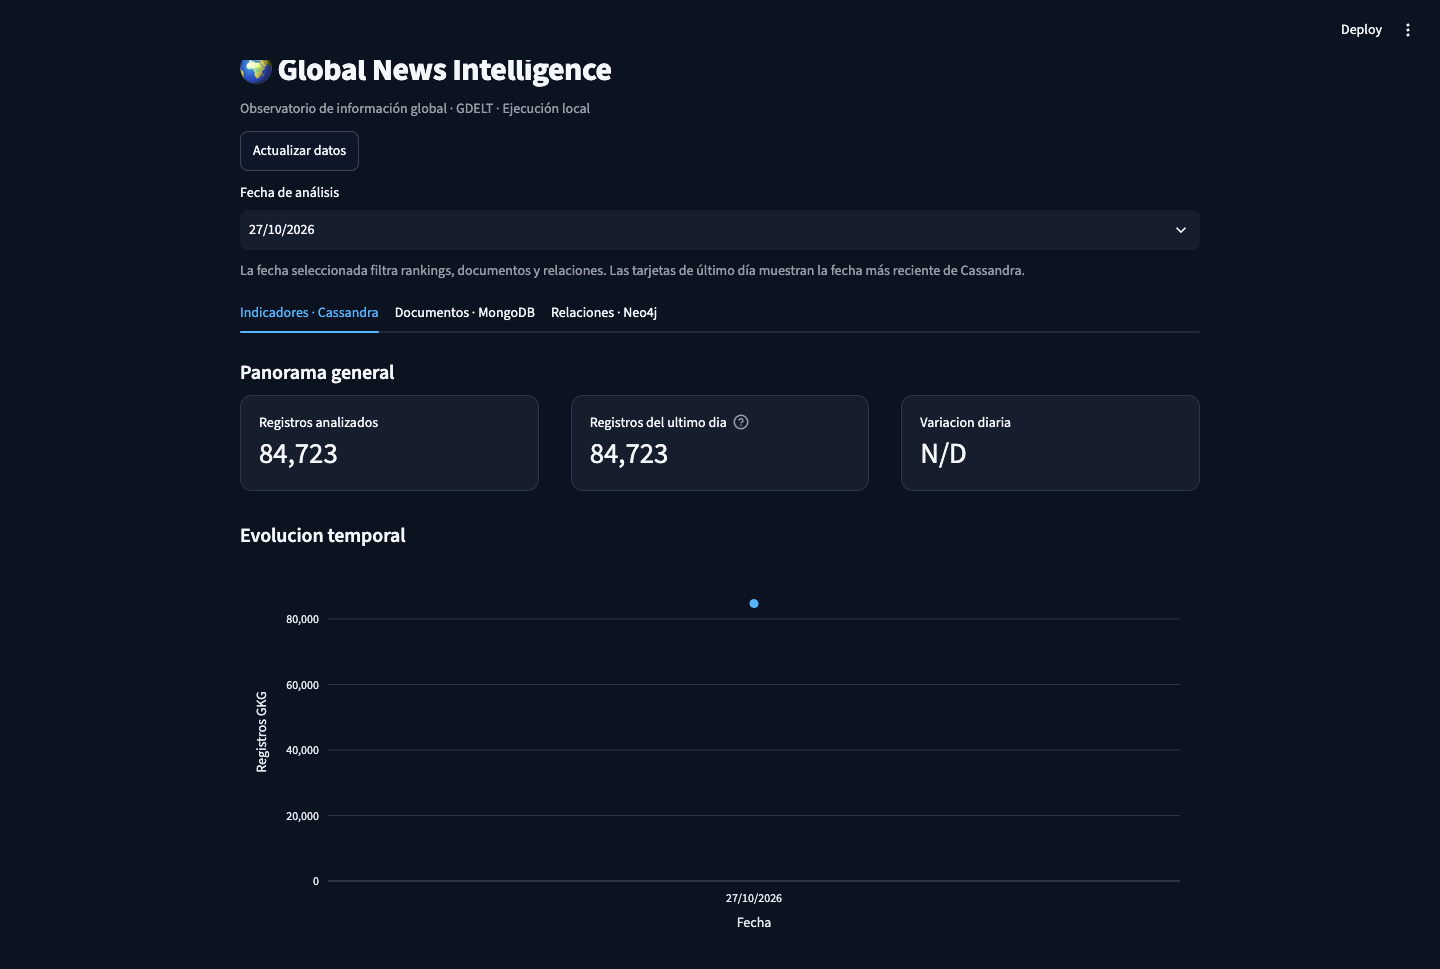
\includegraphics[width=0.85\textwidth]{figs/dash_panorama.png}
\caption{Panorama general: tarjetas de volumen y variación y serie temporal de registros.}
\label{fig:dash-panorama}
\end{figure}

\begin{figure}[H]
\centering
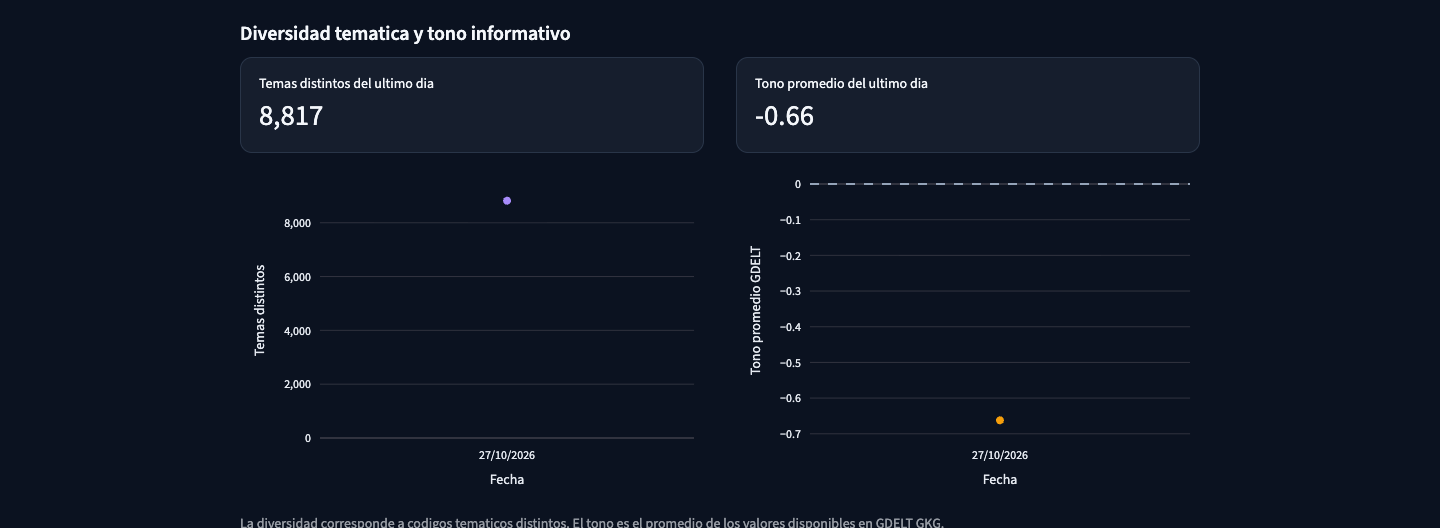
\includegraphics[width=\textwidth]{figs/dash_indicadores.png}
\caption{Diversidad temática y tono informativo, con la línea de tono neutro en cero.}
\label{fig:dash-indicadores}
\end{figure}

\begin{figure}[H]
\centering
\begin{subfigure}{0.49\textwidth}
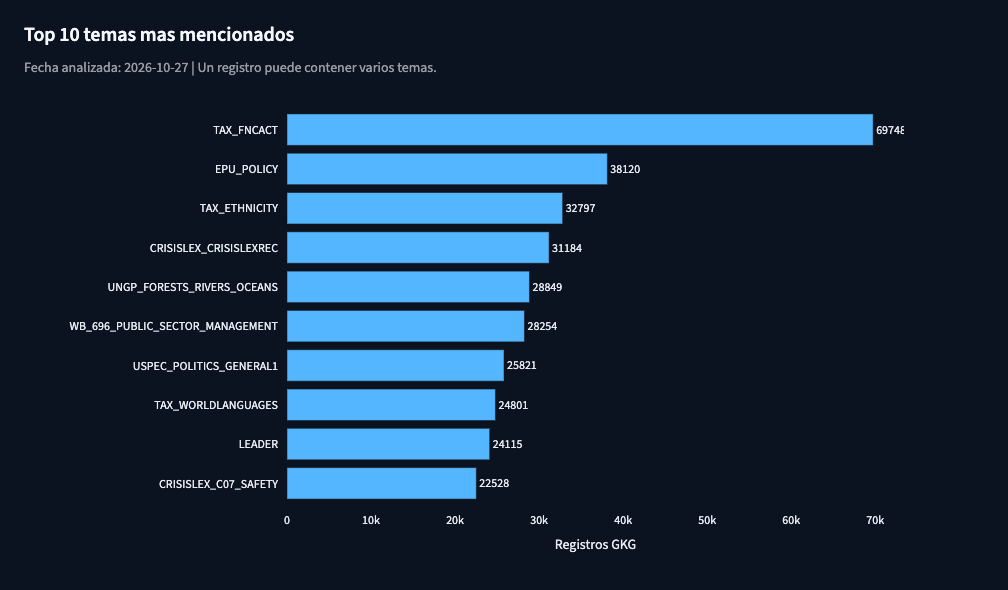
\includegraphics[width=\textwidth]{figs/dash_temas.png}
\caption{Temas más frecuentes.}
\end{subfigure}
\hfill
\begin{subfigure}{0.49\textwidth}
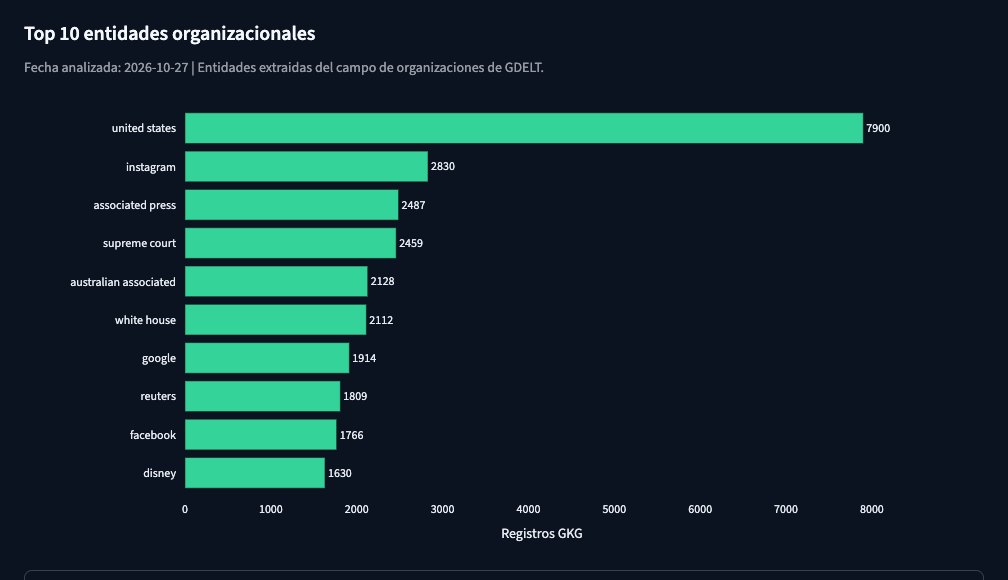
\includegraphics[width=\textwidth]{figs/dash_organizaciones.png}
\caption{Organizaciones más mencionadas.}
\end{subfigure}
\caption{Rankings calculados desde Cassandra para la fecha seleccionada.}
\label{fig:dash-rankings}
\end{figure}

\subsection{Vista documental (MongoDB)}

El explorador documental permite filtrar los registros de una fecha por un código de tema exacto o por una organización que contenga el texto buscado, paginar los resultados y abrir el documento JSON completo.

\begin{figure}[H]
\centering
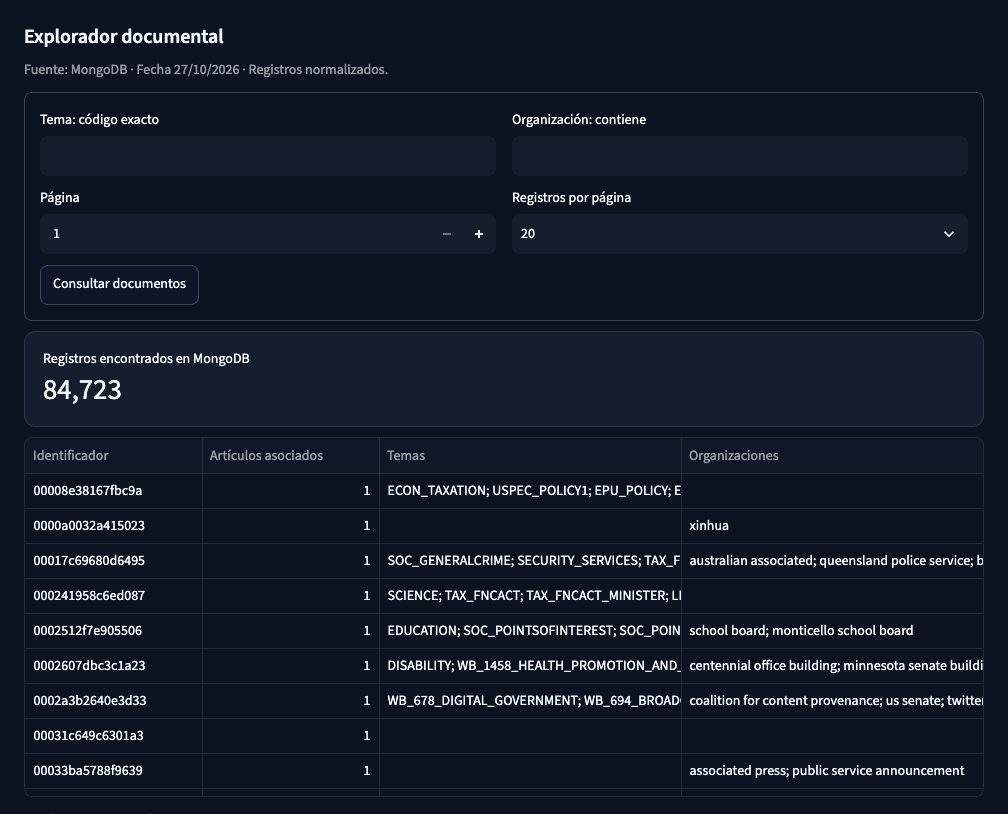
\includegraphics[width=0.75\textwidth]{figs/dash_documentos.png}
\caption{Explorador documental: filtros, conteo de registros encontrados y tabla paginada.}
\end{figure}

\subsection{Vista de relaciones (Neo4j)}

La vista de relaciones muestra los conteos de registros y de relaciones de la fecha y dibuja una muestra del grafo con los temas a la izquierda, los registros al centro y las organizaciones a la derecha.

\begin{figure}[H]
\centering
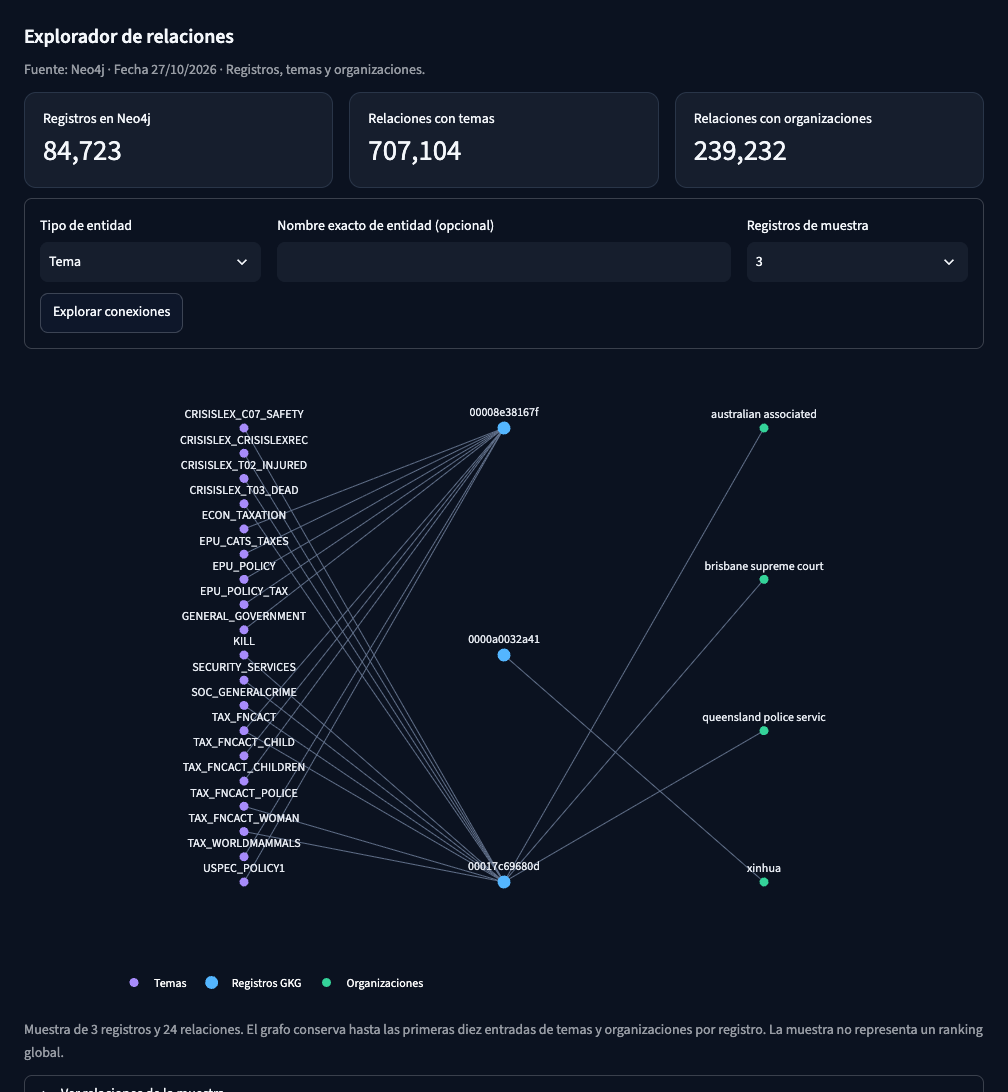
\includegraphics[width=0.75\textwidth]{figs/dash_relaciones.png}
\caption{Explorador de relaciones: conteos del grafo y muestra de tres registros con sus temas y organizaciones.}
\end{figure}

Las capturas corresponden a la fecha de análisis 27 de octubre de 2026. Con el histórico completo, el selector de fecha ofrece las seis fechas cargadas.

% -------------------------------------------------------------
\section{Conclusiones}\label{sec:conclusiones}
% -------------------------------------------------------------

\subsection{Cumplimiento de los objetivos}

\begin{itemize}
    \item Se implementó una arquitectura multimodelo con MongoDB, Cassandra y Neo4j, y cada tipo de dato se justificó por su patrón de acceso.
    \item El DAG de Airflow automatiza las seis etapas del proceso y se verificó con una ejecución programada y con una repetición idempotente.
    \item Se calcularon seis KPIs, por encima del mínimo de cinco, y se reconcilian entre las tres bases.
    \item Las operaciones de creación, consulta, actualización y eliminación se demostraron en las tres bases, incluida la creación y eliminación de una relación en Neo4j.
    \item El tablero consulta las tres bases y se mantiene operativo ante la falla de una de ellas.
\end{itemize}

\subsection{Principales resultados}

El histórico procesado contiene 403\,941 registros en seis fechas, 4\,502\,015 relaciones en el grafo (3\,354\,593 hacia temas y 1\,147\,422 hacia organizaciones) y seis indicadores generados de forma automática. El conjunto cumple el mínimo de 50\,000 registros con un margen de ocho veces. En el entorno de referencia, las 34 pruebas automatizadas se ejecutan con resultado satisfactorio.

\subsection{Dificultades y soluciones}

\begin{itemize}
    \item Publicación consistente en Cassandra: al no haber transacciones entre particiones, una falla podía dejar agregados parciales visibles. Se resolvió con versiones inmutables identificadas por UUID y un puntero que se actualiza al final, y se comprobó con una falla inducida.
    \item Reejecución sin duplicados: se resolvió con identificadores deterministas, \code{upsert} con \code{$setOnInsert} en MongoDB y \code{MERGE} en Neo4j.
    \item Datos voluminosos entre tareas: se evitó enviar archivos por XCom publicándolos como artefactos y transmitiendo solo sus rutas.
    \item Portabilidad de rutas: las URI de artefactos con letra de unidad en Windows se interpretaban como rutas relativas. Se corrigió con la conversión estándar de URI a ruta del sistema y se agregó una prueba.
\end{itemize}

\subsection{Limitaciones y trabajo futuro}

\begin{itemize}
    \item El despliegue es de un solo nodo por base y sin alta disponibilidad. Un entorno productivo requeriría replicación en Cassandra y un clúster de Neo4j.
    \item No se definió una política de retención de las versiones antiguas de Cassandra. Las versiones previas se conservan.
    \item El grafo conserva diez entradas por lista de temas y de organizaciones por registro. Quitar el límite exige evaluar el crecimiento del grafo.
    \item Los rankings se ordenan en la aplicación y no en la base.
    \item El diseño supone archivos diarios inmutables y un único escritor por fecha.
    \item Aún no se han hecho pruebas formales de rendimiento ni se ha reproducido la instalación en una segunda máquina.
    \item Como extensión, entidades como persona, fuente y ubicación podrían promoverse a nodos si aportan preguntas de negocio, con el costo de ampliar la carga, el esquema y el tablero.
\end{itemize}

% -------------------------------------------------------------
\appendix
\section{Estructura del repositorio y ejecución}
% -------------------------------------------------------------

\begin{table}[H]
\centering
\small
\begin{tabular}{@{}ll@{}}
\toprule
Ruta & Contenido \\
\midrule
\path{dags/} & DAG \code{global_news_ingestion} \\
\path{src/ingestion/, validation/, transformation/} & Descarga, validación, transformación y cargas \\
\path{src/pipeline/} & Lógica de las tareas y almacenamiento de artefactos \\
\path{scripts/} & Creación de bases, demostración de CRUD, verificaciones \\
\path{scripts/mongodb/, cassandra/, neo4j/} & Esquemas de cada base \\
\path{dashboard/} & Tablero Streamlit \\
\code{compose.yaml, compose.airflow.yaml} & Despliegue con Docker Compose \\
\path{docs/} & Guías y evidencias de verificación \\
\path{tests/} & Pruebas automatizadas \\
\bottomrule
\end{tabular}
\caption{Estructura principal del repositorio.}
\end{table}

\begin{lstlisting}[language=bash]
python -m venv .venv && source .venv/bin/activate   # Windows: .venv\Scripts\activate
python -m pip install -r requirements-lock.txt
docker compose --env-file .env up -d --wait --wait-timeout 600
python -m scripts.bootstrap_databases
python -m scripts.run_pipeline --date 20261027       # equivale al DAG, en terminal
python -m scripts.crud_demo                          # demostracion de CRUD
streamlit run dashboard/app.py
\end{lstlisting}

\section*{Referencias}

\begin{itemize}[leftmargin=1.2cm, itemsep=4pt]
    \item Apache Software Foundation. (2026). \textit{Apache Airflow 2.11.1 documentation}. \url{https://airflow.apache.org/docs/apache-airflow/2.11.1/}
    \item Apache Software Foundation. (2026). \textit{Apache Cassandra documentation}. \url{https://cassandra.apache.org/doc/latest/}
    \item Leetaru, K., \& Schrodt, P. A. (2013). \textit{GDELT: Global Data on Events, Location and Tone, 1979--2012}. Documento presentado en la ISA Annual Convention. \url{https://www.gdeltproject.org/}
    \item MongoDB, Inc. (2026). \textit{MongoDB manual}. \url{https://www.mongodb.com/docs/manual/}
    \item Neo4j, Inc. (2026). \textit{Neo4j Cypher manual}. \url{https://neo4j.com/docs/cypher-manual/current/}
    \item Streamlit Inc. (2026). \textit{Streamlit documentation}. \url{https://docs.streamlit.io/}
    \item Tamayo, M. K., et al. (2026). \textit{Global News Intelligence} [Repositorio de código fuente]. GitHub. \url{https://github.com/KarolayTamayoH/global-news-intelligence}
\end{itemize}

\end{document}
